\documentclass[a4paper]{article}
\usepackage{amsmath,amssymb}
\usepackage{lmodern}
\usepackage{graphicx}
%\usepackage[left=3cm,right=2cm,top=2cm,bottom=2cm]{geometry}

\title{OT-Analysis : a software for rich analysis of force
	curves when probing living cells with optical tweezers }
\author{Thierry Galliano$^1$, Guillaume Gay$^2$,\\ Laurent Limozin$^1$, Pierre-Henri Puech$^1$}
\date{}



\begin{document}
\maketitle

\noindent $^1$ : Inserm UMR 1067 / CNRS UMR 7333 / AMU UM61 / CENTURI  ; Lab. Adhésion et Inflammation ; Marseille - France

\noindent $^2$ : France Bio Imaging ; Montpellier - France

\section{Summary}\label{summary}

Optical tweezers are a light-based technique for micromanipulating
objects. It allows to move objects such as microbeads and cells, and to record minute forces down to a few pN, which makes it a technique very well adapted to
mechanical measurements on living cells \cite{gennerich_optical_2017}.
We are interested in the mechano-transduction properties of lymphocytes. We seek to dissect the effect of forces and cell mechanics on the
cellular response, in the context of the immune system. T cell mechanotransduction has been
recently demonstrated to be instrumental in the finesse and accuracy of the
response of the latter \cite{puech_mechanotransduction_2021}. Aside,
cells can exert forces when performing their action, eg. cytotoxic T
cells are using forces to kill target infected cells
\cite{basu_cytotoxic_2016}.

Using optical tweezers and specifically decorated beads as handles, we
pull membrane nano-tubes from gently adhered living lymphocytes
\cite{sadoun_dissecting_2020}. Such nanotubes are usually used to
probe the tension of adherent cells \cite{diz-munoz_control_2010}. By
varying the antibodies that are used to decorate the beads, we select
the molecule type we specifically pull on, and we then explore the
molecules which are characteristic of the immune synapse, that is one of
the key organisational structures that has profound implications in T
cell recognition and action \cite{baldari_immune_2017}.

Using this approach, we probe not only the forces of recognition of the
given antibody to its target molecule, but also, by using strong
extracellular bridges, we probe the cytosolic link of the probed molecule
to the cytoskeleton. Such a link has been proposed to be instrumental in
the way T cells can apply or feel forces through the molecule. A
theoretical model has been built and will be reported in a dedicated
article \cite{manca_membrane_2022}. Aside, we will demonstrate the application of the software on full data.

\begin{figure}[h]
	\centering
	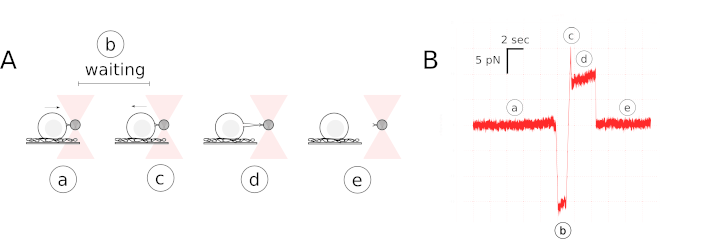
\includegraphics[width=\linewidth]{dessin2}
	\caption{Schematics of the experiment. A : Sequence of events (a) antibody decorated bead,  trapped by the focused infrared laser beam, and lymphocyte are far from each other, and approached ; (b) contact is formed under a controlled level of force and maintained for a given time ; (c) the cell is displaced away from the bead, eventually resulting in the pulling of a tube (d) and its rupture (e), back to the situation of (a). B : Resulting Force vs.Time curve with the indicated events. Adapted from \cite{manca_membrane_2022}}
	\label{fig:dessin}
\end{figure}

The experimentally obtained data consists in force signal as a function of time
(among other parameters), in the three directions of space, obtained in
large quantities (at least 10 per cell / bead couple, and up to 20
couples tested per sample), containing rich and detailled features that
can relate to molecular and/or cellular mechanics that our model
explores. It is therefore needed to standardize and semi-automatize data
analysis to help the experimentalist, often a biologist, to extract
relevant features from the experimental data sets.


\section{Statement of need}\label{statement-of-need}

The avalaible software that comes with the optical tweezers setup
includes a data processing system, with a GUI, that allows the user to
follow pre-defined data processing schemes. Even if it already allows
the typical user to observe, manipulate, quantify and convert to plain
text and images the data, it is closed source and, as such, cannot
receive implementations of novel functions, depending on the
experimentalist needs.

In particular, in regard to the above described application,
the user would have to interact a lot via mouse-clicks and find
alternative use of preexisting data processing functions to perform the
(time) expensive analysis required. This may introduce bias in the
data, which may impair user-to-user data comparison.

Aside, almost none, if any, open source software has been proposed to
the community eg. via GitHub or GitLab for quantifying optical tweezers
experiments with living cells, while some have been proposed for Atomic
Force Microscopy force mode \cite{muller_nanite_2019}, with a modular
capability. Among them, one can find, with the keywords "optical tweezers", on GitHub :
\begin{itemize}
\item https://github.com/ilent2/ott : an Optical Tweezers Toolbox for calculating the torques and forces on a bead in a simulated situation
\item https://github.com/ilent2/tweezers-ml  : an Interactive Optical Tweezers simulation using Machine Learning
\item https://github.com/ghallsimpsons/optical\_tweezers  : set of macros for calibration
\item https://github.com/softmatterlab/OpticalTweezersTutorial : a tutorial
\end{itemize}

% TODO: \usepackage{graphicx} required
\begin{figure}[h]
	\centering
	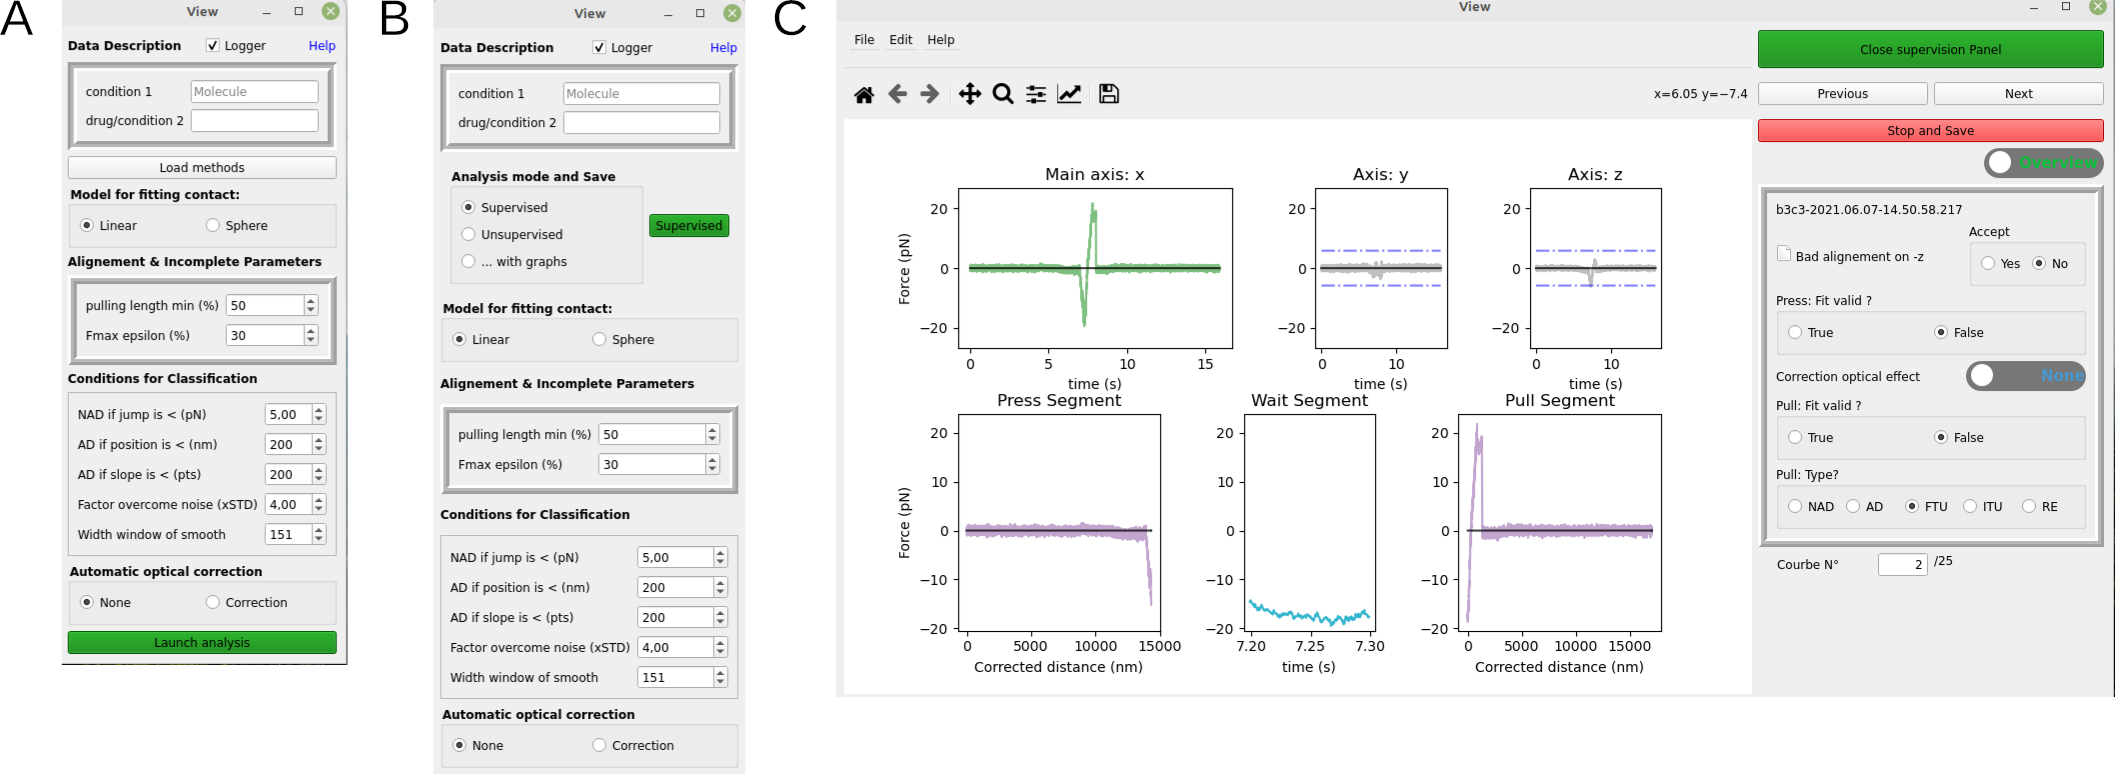
\includegraphics[width=\linewidth]{dessin}
	\caption{Snapshots of OT-Analysis software. A : Starting window where data can be selected and parameters for the analysis set. B : Setting the choice of analysis, from fully automated to user supervised. C : Main window of supervision showing the raw data in the three directions of space, and the results of the pre-analysis, allowing the user to amend the analysis if needed.}
	\label{fig:dessin}
\end{figure}


Of note, OT setups usually allow allows to quantify the forces in the three directions
of space. Thus lateral forces resulting from small geometric mis-alignments
between a given bead and the cell can be probed. As a consequence,
our software has been designed to allow the direct comparison between
these three directions in order to select curves where the force is
detected mainly in one single direction corresponding to the one
selected during the experiment. Aside, we introduced refined baseline
corrections for forces which may be caused, for T cells, by the
deformation of the trap close to contact. We quantify the cell
mechanics, when pushing the bead on the cell, and also cell adhesion or
tube pulling when separating them. Due to the large number of curves
that are typically produced, we implemented data processing by subsets,
in order to be able to use regular or old computers to be able to
distribute it to our students.

We based our software on command line processing functions that we
developed in the lab, and implemented a user friendly, modular, Qt based
GUI which is more than needed when a non code-savy scientist wants to
process complex biological data.

Our resulting software, as such, can serve as a basis for adding new
features in the field of force measurements by optical tweezers.



\section{Acknowledgements}\label{acknowledgements}

We acknowledge data contributions from O. N'Dao, G. Eich, L. Normand. We
also acknowledge the work on a previous Tk based version of the GUI from
K. Himmet. We aknowledge the funding of Labex INFORM (ANR-11-LABX-0054
and AMIDEX project (ANR-11-IDEX-0001-02), funded by the "Investissements d'Avenir" French Government program managed by the
French National Research Agency (ANR)) that allowed LAI to obtain the
optical tweezers set-up, and the continuous help from JPK
instruments/Bruker with it.

\section{References}\label{references}
\bibliographystyle{unsrt} % We choose the "plain" reference style
\bibliography{paper} % Entries are in the refs.bib file

\end{document}
